\section{Tetrahedral microphone array}
A unit vector $\overline{u}$ in 3d space can be defined in spherical coordinates by (1,$\theta$,$\phi$), where the magnitude of the vector is 1, $\theta$ the azimuth and $\phi$ the elevation [3d space point fig here]. We get
\begin{equation}
    \begin{split}
        x_u&=sin(\theta)cos(\phi) \\
        y_u&=sin(\theta)sin(\phi) \\
        z_u&=cos(\theta),
    \end{split}
\end{equation}
this can be denoted by the unit propagation vector ${a(\theta,\phi)}$ in the Cartesian coordinates
\begin{equation}
    a(\theta,\phi)=\begin{bmatrix}sin(\theta)cos(\phi) \\sin(\theta)sin(\phi) \\cos(\theta)\end{bmatrix},
\end{equation}
Suppose sound is travelling along the unit vector $\overline{u}$. Let 2 microphones be placed at positions $\overline{p_1}=(x_1,y_1,z_1)$ and $\overline{p_2}=(x_2,y_2,z_2)$.  Then $\overline{p_{12}}=\overline{p_{2}}-\overline{p_{1}}$, where ${\overline{p_{12}}}$ is the distance between the two microphones. The projection of this distance in the direction of $\overline{u}$ is simply $a(\theta,\phi)\overline{p_{12}}$ and the time it takes for sound to travel between the two microphones is then 
\begin{equation}
    T_{12}=\frac{a(\theta,\phi)\overline{p_{12}}}{c},
\end{equation} c being the speed of sound. For 4 microphones, a Least-Squares approach could be considered, with $^4C_2$ combinations possible. The 'correct' DOA is then the $a(\Theta,\Phi)$ which minimizes the cost function
\begin{equation}
    J(\Theta,\Phi) = \sum\bigg(T_{ij}-\frac{a(\Theta,\Phi)\overline{p_{ij}}}{c}\bigg)^2, \text{for } i,j \in \begin{pmatrix}4\\2\end{pmatrix}.
\end{equation}

Using atleast 4 microphones a spatial array can be constructed. The simplest spatial structure with 4 vertices is a tetrahedron (a triangular pyramid). The tetrahedron has 4 vertices, 4 faces and 6 edges. If the tetrahedron is regular then all the vertices are equally spaced from each other and every face is an equilateral triangle.The following section discusses the simulated performance of different TDOA and DOA algorithms on a tetrahedral array in an outdoor environment.

\subsection{Regular tetrahedral array}

%Let's define a regular tetrahedral array geometry as follows
%\begin{equation}
%    \begin{split}
%        p_1 &= \begin{bmatrix}{-0.5} & {0} & {0}\end{bmatrix}^T \\
%        p_2 &= \begin{bmatrix}{0.5} & {0} & {0}\end{bmatrix}^T \\
%        p_3 &= \begin{bmatrix}{0} & {\sqrt{(0.75)}} & {0}\end{bmatrix}^T \\
%        p_4 &= \begin{bmatrix}{0} & {\sqrt{(0.75)/2}} & {\sqrt{(0.5)}}\end{bmatrix}^T,
%    \end{split}
%\end{equation}


\begin{figure}[H]
    \centering
    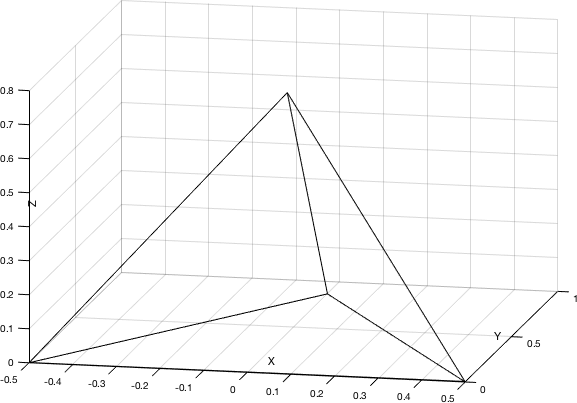
\includegraphics[width=0.7\textwidth]{Figures/regulartetra.png}
    \caption{Representation of a regular Tetrahedral geometry}
    \label{fig:regulartetra}
\end{figure}

The distance between the microphones (array aperture) for the tetrahedron in Fig. \ref{fig:regulartetra} is 1m. For such an array, spatial aliasing would occur for frequencies $> (c*1m)/2 \approx $170Hz, c being the speed on sound.  When Fourier based techniques are used for non-stationary signal, the spatial frequency must satisfy the Nyquist Frequency (i.e be $< c/2$) but this requirement can be relaxed for a stationary signal by using anti-aliasing techniques \cite{dmochowski2009spatial}. Fig. \ref{fig:directivityregulartetra} shows the directivity of a tetrahedral array for various frequencies. As expected, aliasing occurs and the main lobe disappears for frequencies $> c/2$. Fig. \ref{fig:directivityothers} shows the directivity for a 4-element uniform linear array (ULA) and uniform circular array (UCA) with the same array aperture of 1m. Since no elevation information can be retrieved from a uni-dimensional linear array the directivity pattern is donut shaped, meaning that the source is located somewhere on the donut. 


\begin{figure}[H]
\centering
\begin{subfigure}{.5\textwidth}
    \centering
        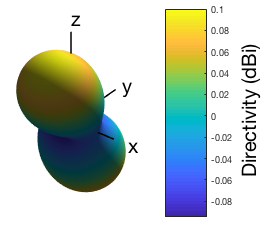
\includegraphics[width=0.7\textwidth]{Figures/regulartetra50hzdirectivity.png}
    \label{fig:directivity200hzregulartetra}
\end{subfigure}%
\begin{subfigure}{.5\textwidth}
        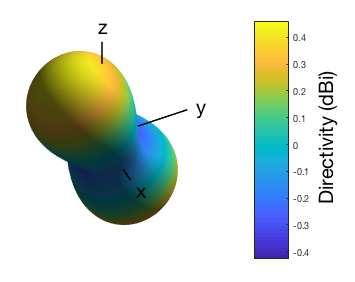
\includegraphics[width=0.7\textwidth]{Figures/regulartetra100hzdirectivity.png}
    \label{fig:directivity100hzregulartetra}
\end{subfigure}
\begin{subfigure}{.5\textwidth}
    \centering
        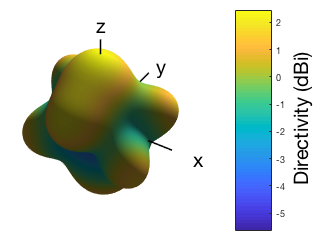
\includegraphics[width=0.9\textwidth]{Figures/regulartetra200hzdirectivity.png}
    \label{fig:directivity200hzregulartetra}
\end{subfigure}%
\begin{subfigure}{.5\textwidth}
    \centering
        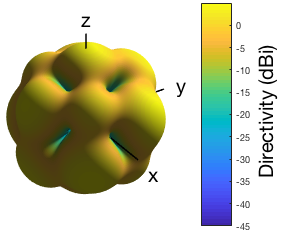
\includegraphics[width=0.9\textwidth]{Figures/regulartetra400hz.png}
    \label{fig:directivity400hzregulartetra}
\end{subfigure}
\caption{Directivity of the regular tetrahedral array at 50hz (top), 100hz(right), 200hz (bottom left) and 400hz (bottom right)}
\label{fig:directivityregulartetra}
\end{figure}


\begin{figure}[H]
\centering
\begin{subfigure}{.5\textwidth}
    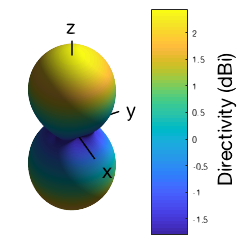
\includegraphics[width=0.85\textwidth]{Figures/uca100hzdirectivity4mic.png}
    \label{fig:directivity100hzuca}
\end{subfigure}%
\begin{subfigure}{.5\textwidth}
    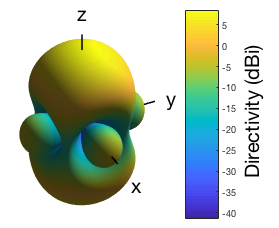
\includegraphics[width=0.85\textwidth]{Figures/uca200hzdirectivity4mic.png}
    \label{fig:directivity100hzuca}
\end{subfigure}%
\caption{Directivity of the UCA array at 100hz(left) and 200hz (right)}
%\label{fig:test}
\end{figure}

\begin{figure}[H]
\centering
\begin{subfigure}{.5\textwidth}
    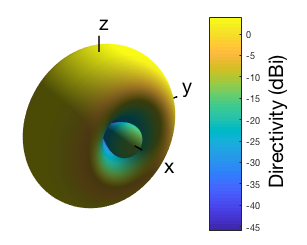
\includegraphics[width=0.85\textwidth]{Figures/ula100hzdirectivity.png}
    \label{fig:directivity100hzuca}
\end{subfigure}%
\begin{subfigure}{.5\textwidth}
    \centering
    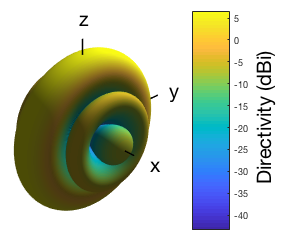
\includegraphics[width=1.1\textwidth]{Figures/ula200hzdirectivity.png}
    \label{fig:directivity100hzula}
\end{subfigure}
\caption{Directivity of the ULA array at 100hz (left) and 200hz (right)}
\label{fig:directivityothers}
\end{figure}